\documentclass[fr,license=none]{../../../eplsummary}

\usepackage{../../../eplcode}

\lstset{language={Oz},morekeywords={for,do,lazy}}

\newcommand{\st}{\mathrm{ST}}
\newcommand{\ce}{\mathrm{CE}}
\newcommand{\mozart}{Mozart}

\usepackage{pgf}
\usepackage{tikz}
\usepackage{circuitikz}
\usetikzlibrary{arrows,automata, shapes, positioning}
\usetikzlibrary{positioning}

\tikzset{
  state/.style={
    rectangle,
    rounded corners,
    draw=black, very thick,
    minimum height=2em,
    inner sep=2pt,
    text centered,
    text width=2.5cm,
  },
  bad/.style={
    state,
    draw=dkred,
  },
  good/.style={
    state,
    draw=dkgreen,
  },
}

\hypertitle{Concepts des languages informatiques}{6}{INGI}{1131}
{Benoît Legat\and Arnaud Schils}
{Peter Van Roy}

\paragraph{Prérequis} Ce cours comporte ``Informatique 2'' en prérequis qui donne une introduction à \oz{}.
Vous êtes invités à lire la synthèse de ce cours si ce n'est déjà fait.

\part{Programmation avancée en \oz{}}
La \figuref{paradigms} reprend les paradigmes abordés par ce cours.
Ceux en rouge sont les paradigmes qui sont à éviter contrairement à ceux en vert qui sont des bons paradigmes.

\begin{myfig}{paradigms}{Paradigmes du cours.}
  \begin{tikzpicture}[->,>=stealth',node distance=3cm]
    \node[state,text width=3cm] (FUNCTIONAL)
    {functional programming};
    \node [yshift=0.5cm,right of=FUNCTIONAL]
    {\(\begin{cases}
        \text{recursion}\\\text{higher-order}
      \end{cases}\)
    };

    \node[good,
      below of=FUNCTIONAL,
      xshift=-5cm,
      anchor=center] (DATAFLOW)
    {deterministic dataflow};

    \node[bad,
      below of=FUNCTIONAL] (EVENTLOOP)
    {event loop programming};

    \node[state,
      below of=FUNCTIONAL,
      xshift=5cm,
      anchor=center] (OOP)
    {sequential OOP};
    \node[yshift=0.5cm,right of=OOP,node distance=2cm] {\sc Java};

    \node[state,
      below of=DATAFLOW,
      anchor=center] (LAZY)
    {Lazy deterministic dataflow};
    \node[below of=LAZY,anchor=east,node distance=1cm] {\sc Haskell};

    \node[good,
      below of=EVENTLOOP,
      anchor=center] (AGENT)
    {Multi-agent dataflow};
    \node[below of=AGENT,anchor=east,node distance=1cm] {\sc Erlang};

    \node[bad,
      below of=OOP,
      anchor=center] (CONCOOP)
    {concurrent OOP};

    \node[good,
      below of=AGENT,
      xshift=2.5cm,
      anchor=center] (ACTIVE)
    {Active objects};
    \node[yshift=0.5cm,right of=ACTIVE,node distance=2cm] {\sc Scala};

    \path
    (FUNCTIONAL) edge node[anchor=south,above,sloped] {$+$ thread}  (DATAFLOW)
    (FUNCTIONAL) edge node[anchor=south,above,sloped] {$+$ port}    (EVENTLOOP)
    (FUNCTIONAL) edge node[anchor=south,above,sloped] {$+$ cell}    (OOP)
    (DATAFLOW)   edge node[anchor=south,above,sloped] {$+$ by-need} (LAZY)
    (EVENTLOOP)  edge node[anchor=south,above,sloped] {$+$ thread}  (AGENT)
    (OOP)        edge node[anchor=south,above,sloped] {$+$ thread}  (CONCOOP)
    (AGENT)      edge node[anchor=south,above,sloped] {$+$ cell}    (ACTIVE)
    (CONCOOP)    edge node[anchor=south,above,sloped] {$+$ ports}   (ACTIVE);
  \end{tikzpicture}
\end{myfig}

\section{Fonctions lazy}
Lazy signifie paresseux en français.
Une fonction lazy est une fonction qui ne va calculer son résultat qu'à partir du moment où on demande vraiment la valeur de son résultat.
La demande de la valeur d'une variable se fait avec la fonction \lstinline|Wait|.
Les opérateurs comme \lstinline|+|, \lstinline|mod|, \lstinline|==| ou même le \lstinline|case| font déjà le \lstinline|Wait| automatiquement.
Les moments où la valeur d'une variable est demandée sont ces moments où le thread seraient bloqués si elle n'avait pas encore de valeur.
C'est d'ailleurs pour ça que la fonction, bien que paresseuse, se décide enfin à calculer son résultat, parce qu'un autre thread est bloqué à cause d'elle.

Pour définir une fonction lazy, on rajoute le \keyword{} lazy après \lstinline|fun|.
Par exemple, le code suivant pourrait être le code de Deep Thought et expliquerait le délais de 7.5 millions d'années pour calculer
la réponse à la vie, l'univers et le reste.
Il faut noter que \lstinline|Browse| ne fait pas de \lstinline|Wait| (s'il le faisait, on aurait du attendre moins longtemps),
il va simplement afficher un underscore en attendant que la variable ait une valeur.
\begin{lstlisting}
declare
fun lazy {Answer}
  42
end
Ans = {Answer}
{Browse Ans}
{Delay 9855000000000000}
{Wait Ans}
\end{lstlisting}

Il est important aussi de noter qu'une fonction lazy s'exécute automatiquement dans un autre thread, sinon
ce code bloquerait à la ligne 5, puisque la fonction attendrait qu'on attende la valeur de \lstinline|Ans| pour continuer.
La traduction en langage noyau de ce code est d'ailleurs
\begin{lstlisting}
declare
proc lazy {Answer ?X}
  thread
    {WaitNeeded X}
    X = 42
  end
end
{Answer Ans}
{Browse Ans}
{Delay 9855000000000000}
{Wait Ans}
\end{lstlisting}

On peut remarquer qu'écrire \lstinline|proc lazy| n'aurait pas de sens car une procédure n'a pas de résultat bien défini donc lors de la traduction
en langage noyau, on ne saurait quelle variable attendre.

\section{Producer-Consumer}
\subsection{Eager}
Producer makes new elements and can get ahead of the consumer.
\begin{description}
	\item[Pros] Fast
	\item[Cons] Risk of memory leak (new elements will pile up).
\end{description}
\subsection{Lazy}
Consumer asks for new element.
Producer only produces when asked.
\begin{description}
	\item[Pros] No leak
	\item[Cons] Reduction of performance
\end{description}
\subsection{Bounded Buffer (BB)}
Buffer with fixed size (N elements) linking the producer to the consumer.
Working eagerly while not full and working lazily while full.
Producer and consumer executed in paralel.
%\begin{description}
%  \item[Eager producer-consumer]
%    Le producteur produit autant qu'il veut et le consommateur consomme ce qu'il produit et attend si le buffer est vide.
%    \textbf{Problème:} Le producteur peut causer un memory overflow.
%  \item[Lazy producer-consumer]
%    Le producteur attend que le consommateur demande un élément pour le produire.
%    \textbf{Problème:} Le consommateur doit attendre pour chaque élément.
%  \item[Bounded buffer]
%    Pareil que ``Eager producer-consumer'' mais le buffer a une taille limitée.
%\end{description}

\section{Deterministic dataflow}
The expression \textbf{declarative concurrency} seems to represent the same paradigm.
Declarative programming = functional programming. A program is a mathematical function (deterministic).
Deterministic dataflow is more general than just functional programming :
\begin{itemize}
	\item concurrent/long lived, streams
	\item unbound variables
\end{itemize}
\subsection{Definition of declarative concurrency}
A program is declarative if for all possible inputs, all executions for a particular input:
\begin{itemize}
	\item whether all do not terminate 
	\item whether all event reach partial termination and outputs are logically equivalent.
\end{itemize} % both conditions should be true or one of the 2?

All deterministic and lazy deterministic dataflow programs are declarative.
\subsection{Avantages du deterministic dataflow}
\begin{itemize}
  \item Tous les programmes fonctionnels peuvent devenir concurrents.
  \item Les résultats ne changent pas quand on ajoute des threads.
  \item Les calculs deviennent incrémentaux.
  \item On construit des programmes avec des streams qui sont
    des listes sans fin (ça donnera lieu aux stream objects et stream agents).
\end{itemize}
\subsection{Limitations du deterministic dataflow}
Its determinism.
\begin{itemize}
  \item same inputs give same (or equivalent) results (eventually).
  \item when the execution stops for a given input, the outputs are equivalent.
\end{itemize}

Il y a beaucoup de programmes qui doivent avoir un comportement non-déterministe.
Par exemple, une application client-serveur avec au moins 2 clients.
Le comportement de l'application dépend de l'ordre dans lequel le serveur reçoit les messages des clients, ce n'est donc pas déterministe.  Il y a besoin d'introduire la notion de choix (non déterministe).
\begin{lstlisting}
declare
proc {Server S1 S2}
  C={WaitTwo S1 S2} % -> Choice
  ...
end
\end{lstlisting}
Pour résoudre cela, on introduit les ports.

\subsection{Objets}
Différents types d'objets
\begin{itemize}
  \item Stream objects
  \item Port objects
  \item Passive objects : cells (attributes) + data (values) (Java)
  \item Active objects = Passive object + threads (port).
\end{itemize}

\section{Ports}
Message protocols
\begin{itemize}
  \item RMI
  \item asynchronous RMI
  \item RMI with callback
\end{itemize}

\section{Shared-State Concurrency}
Introduction of the cells.
Multiples threads share a state and have operations.
Suppose thread T1 having operations $a_1 \ a_2 \ a_3 ... \ a_k$ and thread T2 having operations $b_1 \ b_2 \ b_3 ... \ b_k$ on the cell C.
There happen conflicts (interleavings). Cell c sees $ a_1 \ a_2 \ b_1 \ a_3 \ ...$ Many possible interleavings exists : 
$2k! / k!$
All interleavings should be correct.

Il y a 3 instructions atomiques,
\lstinline|@|, \lstinline|:=| et \lstinline|Exchange|.
\subsection{Managing the interleaving}
\subsubsection{Locks}
A lock protects a region of code. Only one thread can execute inside at any moments.
\begin{lstlisting}
L={NewLock}
lock L then 
	_ %New syntax
	_
	_
	_
end
\end{lstlisting}
\begin{lstlisting}
local X Y in
	Y=@C
	C:=X
	{Wait Y}
	_
	_
	_
	X=ok
end
\end{lstlisting}

To make a lock, we need an atomic read+write operation combining the operations of reading and writing the cell.  This operation must be provided by the system.  All processors provide atomic read+write. In oz, it is provided by the function {Exchange C Y X} where Y is bound to the current content of C and X is the new content of C.

Locks are not enough $\rightarrow$ Bounded Buffer.
\subsubsection{Monitors}
2(3) new operators :
\begin{itemize}
	\item wait : suspend current thread. put it in wait set, release the lock.
	\item notify : 
	\begin{enumerate}
		\item remove a thread from wait set
		\item the thread start executing : it first tries to get the lock at the point where it was suspended.
	\end{enumerate}
	\item notifyAll: like notify but all thread are removed.
\end{itemize}

Programming patterns for monitors :
\begin{lstlisting}
meth methname(...)
	lock
	while not cond do wait
		%Code
	notifyAll
	end
end
\end{lstlisting}
\subsection{Transactions}
Motivation : Accessing to a database (array of cells).
\begin{itemize}
	\item Performance
	\item Scalability
	\item Fault tolerance (if crash, coherent stop).
\end{itemize}
Different solutions :
\subsubsection{Naive version}
One lock for all the database.
$\rightarrow$ Very slow, not scalable.
\subsubsection{One lock by cell in DB}
\begin{itemize}
	\item allows parallelism
	\item scalable
	\item real DB
\end{itemize}
\vspace{0.5cm}
%il doit exister une meilleure manière de dessiner cela mais je ne suis pas expérimenté à ce niveau ^^.
\begin{circuitikz} \draw %Graphe Thread T1
(0,0.25) node[] {T1}
(1.5,0) node[] {$C_a$}
(5.25,0) node[] {$C_b$}
(0,0) -- (1,0)
(1,0) -- (1,0.5)
(1,0.5) -- (1.75,0.5)
(1.75, 0.5) -- (1.75,0)
(1.75,0) -- (4.75,0)
(4.75,0) -- (4.75, 0.5)
(4.75, 0.5) -- (5.5, 0.5)
(5.5,0.5) -- (5.5,0)
(5.5,0) -- (7,0)
;
\end{circuitikz}
\newline
\vspace{0.5cm}
\begin{circuitikz} \draw %Graphe Thread T2
(0,0.25) node[] {T2}
(2.5,0) node[] {$C_a$}
(4,0) node[] {$C_b$}
(0,0) -- (2.25,0)
(2.25,0) -- (2.25,0.5)
(2.25,0.5) -- (3,0.5)
(3, 0.5) -- (3,0)
(3,0) -- (3.5,0)
(3.5,0) -- (3.5, 0.5)
(3.5, 0.5) -- (4.25, 0.5)
(4.25,0.5) -- (4.25,0)
(4.25,0) -- (7,0)
;
\end{circuitikz}
\newline
There can be interference if the transactions T1 and T2 want to access to cells $C_a$ and $C_b$.  T2 doesn't see the modification of $C_b$ in T1, too late. T1, T2 not serializable : T1 or T2 before T1.

How can we make the problem serializable?
With 2 phase locking :
\begin{enumerate}
	\item We get locks
	\item We release locks
\end{enumerate}
If we use 2PL to get locks then transactions are serializable.
But what if a transaction abort?
We need to release all locks at once.

\textbf{Strict 2PL}: serializable transactions without cascading abort.
\textbf{Deadlock}: ressource conflicts in any system with agents(threads running transactions) and resources (locks).
\newline
\begin{circuitikz} \draw
(0,0.25) node[] {T1}
(2.25,0) node[] {$C_a$}
(5,0.5) node[] {need $C_b$ ?}
(0, 0) -- (2,0)
(2,0) -- (2,0.5)
(2,0.5) -- (4, 0.5)
;
\end{circuitikz}
\newline
\begin{circuitikz} \draw
(0,0.25) node[] {T2}
(2.25,0) node[] {$C_b$}
(5,0.5) node[] {need $C_a$ ?}
(0, 0) -- (2,0)
(2,0) -- (2,0.5)
(2,0.5) -- (4, 0.5)
;
\end{circuitikz}
\newline
If this situation happens, both threads will wait forever! $\rightarrow$ Circular wait between threads that need resources : deadlock.
\subsubsection{Wait for graph}
\begin{center}
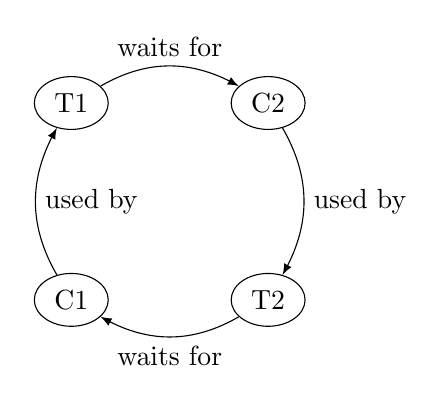
\begin{tikzpicture}[on grid, auto]
    \node[draw, ellipse] (A) {T1};
    \node[draw, ellipse] (B) [right = 2.5 cm of A] {C2};
    \node[draw, ellipse] (C) [below = 2.5 cm of B] {T2};
    \node[draw, ellipse] (D) [below = 2.5 cm of A] {C1};

    \path[-latex] (A) edge [bend left] node [above] {waits for} (B);
    \path[-latex] (B) edge [bend left] node [right] {used by} (C);
    \path[-latex] (C) edge [bend left] node [below] {waits for} (D);
	\path[-latex] (D) edge [bend left] node [right] {used by} (A);
\end{tikzpicture}
\end{center}
In a wait for graph, we represent the relations between the transactions and Cells (protected by a lock). There are only 2 kind of nodes in this graph : used by and waits for. 
\subsubsection{Concurrency control}
Need of concurrency control(CC) : 
\begin{itemize}
	\item techniques used to implement transaction
	\item strict 2PL part of CC
	\item in a system : Transaction manager
\end{itemize}
\subsubsection{Transaction manager (TM)}
A transaction asks for a lock :
The transaction manager either :
\begin{itemize}
	\item gives the lock
	\item doesn't give the lock
	\item delays
\end{itemize}
If the TM is optimistic, it gives even if it's risky.
If the TM is pessimistic, it delays if it's risky.
\newline
\textbf{Naive TM} :
\begin{itemize}
	\item if transaction asks for unlocked cell : give the lock.
	\item STRICT 2PL : only allowed to release after all gets.
\end{itemize}
\textbf{Deadlock repair} :
Detect cycle in wait for graph.
if cycle found, choose one transaction and restart it (abort by releasing all locks, and start again).
\newline
\textbf{Deadlock avoidance} :
If we give priorities to transactions and give higher priorities to earlier transactions, when transaction asks for a lock on a cell :
\begin{itemize}
	\item unlocked : it gets the lock
	\item locked by actual transaction : continue
	\item locked by higher priority transaction : waits
	\item locked by lower priority transaction : low priority transaction restarts and release all its locks.
\end{itemize}
\vspace{1cm}
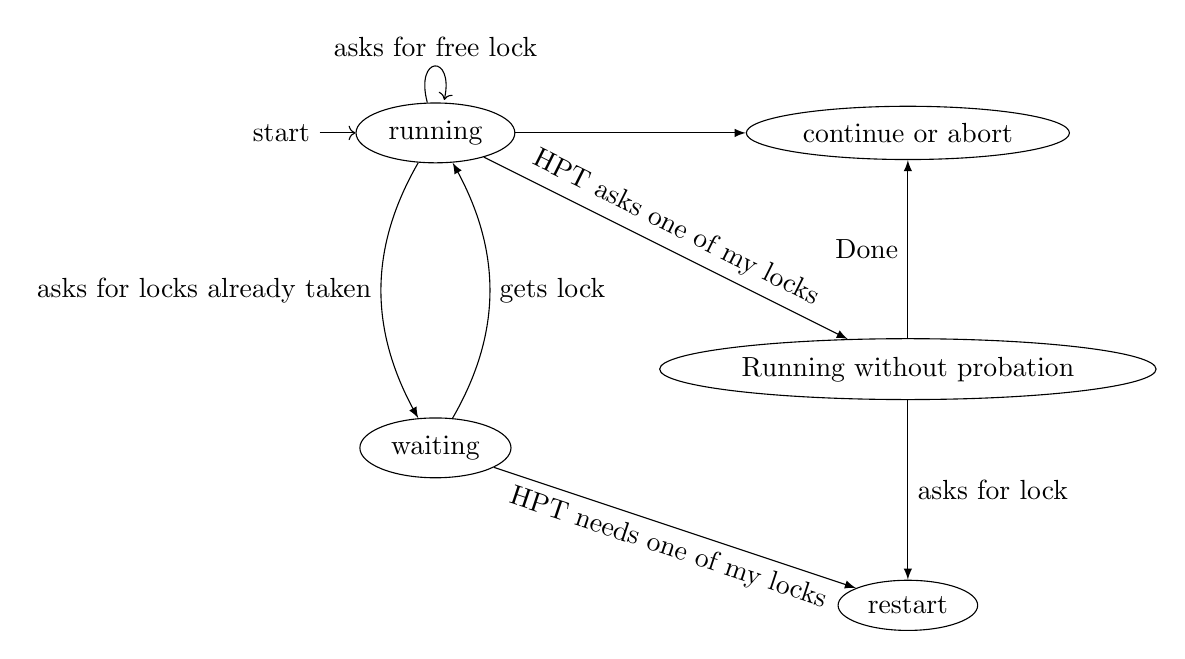
\begin{tikzpicture}[on grid, auto]
    \node[initial,draw, ellipse] (A) {running};
    \node[draw, ellipse] (B) [right =6 cm of A] {continue or abort};
    \node[draw, ellipse] (C) [below =3cm of B] {Running without probation};
    \node[draw, ellipse] (D) [below =4cm of A] {waiting};
    \node[draw, ellipse] (E) [below = 3cm of C] {restart};

    \path[-latex] (A) edge [loop above] node {asks for free lock} (A);
    \path[-latex] (A) edge [bend right] node [left] {asks for locks already taken} (D);
    \path[-latex] (D) edge [bend right] node [right] {gets lock} (A);
    \path[-latex] (A) edge node {} (B);
    \path[-latex] (A) edge node[sloped, anchor=center,above] {HPT asks one of my locks} (C);
    \path[-latex] (C) edge node {Done} (B);
    \path[-latex] (C) edge node {asks for lock} (E);
    \path[-latex] (D) edge node[sloped, anchor=center,below] {HPT needs one of my locks} (E);
\end{tikzpicture}
\newline
HPT = higher priority transaction
The part "Running without probation" is an additional part for optimisation.
\clearpage
\part{Définitions}
Ceci est une liste exhaustive constituée par Arnaud Schils
des définitions du livre
``Concepts, Techniques and Models of Computer Programming''
complètée avec ses notes de cours.
%    ________________________________________________
%   / ____        __ _       _ _   _                 \
%  / |  _ \  ___ / _(_)_ __ (_) |_(_) ___  _ __  ___  \
% |  | | | |/ _ \ |_| | '_ \| | __| |/ _ \| '_ \/ __|  |
% |  | |_| |  __/  _| | | | | | |_| | (_) | | | \__ \  |
%  \ |____/ \___|_| |_|_| |_|_|\__|_|\___/|_| |_|___/ /
%   \------------------------------------------------/
%     \               ,-----._
%   .  \         .  ,'        `-.__,------._
%  //   \      __\\'                        `-.
% ((    _____-'___))                           |
%  `:='/     (alf_/                            |
%  `.=|      |='                               |
%     |)   O |                                  \
%     |      |                               /\  \
%     |     /                          .    /  \  \
%     |    .-..__            ___   .--' \  |\   \  |
%    |o o  |     ``--.___.  /   `-'      \  \\   \ |
%     `--''        '  .' / /             |  | |   | \
%                  |  | / /              |  | |   mmm
%                  |  ||  |              | /| |
%                  ( .' \ \              || | |
%                  | |   \ \            // / /
%                  | |    \ \          || |_|
%                 /  |    |_/         /_|
%                /__/

\section{Chapters 4.1 to 4.6 and 4.8}

\subsection{4.1 The data-driven concurrent model}

\begin{description}
  \item[Thread] semantic stack, sequence of instructions that executes (sequential).
    Threads of a same program share address space.
  \item[Agent] tail-recursive list function executing in a thread.
  \item[Data-driven concurrent model] declarative model + threads.
    \begin{itemize}
      \item keeps all the good properties of the declarative model.
      \item 2 differences with functional programming:
        \begin{enumerate}
          \item Inputs and outputs are not necessarily values, they can contain unbound variables.
          \item Execution might not terminate since the inputs can be streams that grow indefinitely.
        \end{enumerate}
    \end{itemize}

  \item[Lazy concurrent model] data-driven concurrent model + ``by need triggers''
    \begin{itemize}
      \item possibility to do demand-driven computation or lazy execution.
      \item keeps also good properties of the declarative model.
    \end{itemize}
  \item[Nondeterminism] there is an execution state in which there is a choice of what to do next (ex: which thread to reduce?).
    The choice is made by the system.
    \begin{itemize}
      \item Observable nondeterminism can give different results (race condition).
      \item Not observable $\rightarrow$ same results.
    \end{itemize}
  \item[Scheduler] part of the system, choose the next thread to execute.
    It chooses which semantic stack execute according to a well defined set of rules called the ``scheduling algorithm''.
    \begin{description}
      \item[Scheduling algorithm] this algorithm is careful to make sure that good properties (fairness) hold for any computation.
      \item[Round-robin scheduling] Scheduler puts all ready threads in a queue.
        At each step, it takes the first thread out of the queue, lets it execute some numbers of steps, and then puts it back in the queue.
        It guarantees that processor time is spread out equitably over the ready threads.
      \item[Time slices] each thread has a maximum time that it is allowed to run before the scheduler stops it.
        This time interval is called time slice.
      \item[Preemption] stopping a running thread in the ``time slice out'' way.
      \item[Counting approach] count computation steps and give the same number to each thread.
        Scheduler execution is deterministic.
      \item[Timer approach] use a hardware timer that gives the same time to each thread.
        More efficient (supported by hardware), scheduler is no longer deterministic.
    \end{description}
  \item[Ready / runnable thread] a thread is ready if its statement has all the information it needs to execute at least one computation step.
  \item[Not ready / suspended / blocked thread] it does not have all the information it needs.
    We say its first statement is blocked.
  \item[Execution tree] summary of all possible executions.
  \item[Partial termination] a program does a partial termination if it hasn't terminated completely yet, since further binding the inputs would cause it to execute further.
    If the input do not change, then the program will execute no further.
  \item[Declarative concurrent program] a program is concurrent declarative if for all possible inputs, all executions with a given set of inputs have one of two results:
    \begin{itemize}
      \item they all do not terminate.
      \item they reach a partial termination and give results that are logically equivalent.
    \end{itemize}
    There is no observable nondeterminism.
  \item[Failure] abnormal termination of a declarative program that occurs when we attempt to put conflicting information in the store.
\end{description}

\subsection{4.2 Basic thread programming techniques}

\begin{description}
  \item[Priority levels] each priority level is given a minimum percentage of the processor time.
    Within each priority level, threads share the processor time fairly as before.
    There are queues for each priority level.
  \item[Cooperative concurrency] entities that are working together on some global goal (threads).
  \item[Competitive concurrency] entities have a local goal, working just for themselves.
    Interested  only in their own performance.
    (process managed by the operating system).
\end{description}

\subsection{4.3 Streams}

\begin{description}
  \item[Stream] potentially unbounded list of messages.
    List whose tail is an unbound dataflow variable.
    The most useful technique for concurrent programming in the declarative concurrent model is using streams to communicate between threads.
  \item[Deterministic stream programming] each stream object always knows for each input where the next message will come from.
  \item[Producer] thread creating a stream incrementally by binding the tail to a new list pair and a new tail.
  \item[Comsumer] read the producer's stream.
    Because the stream's tail is a dataflow variable, the consumers will read the stream as it is created.
  \item[Transducer] object between the producer and the consumer.
    It reads the producer's stream and creates another stream which is read by the consumer.
  \item[Pipeline] sequence of stream objects each of which feeds the next.
  \item[Flow control] limit the rate at which the producer generates new elements.
    It requires that some information be sent back from the consumer to the producer.
    \begin{description}
      \item[with demand-driven concurrency] the producer only generates elements when the consummer explicitly demandes them.
        We can use dataflow for the consumer to signal the producer whenever it needs a new element.
        This implements lazy execution.
        Strong reduction in throughput.
      \item[with a bounded buffer] combination of eager and lazy execution.
        A bounded buffer is a tranducer that stores elements up to a maximum number.
        The producer is allowed to get ahead of the consumer, but only until the buffer is full.
        This limits the extra ressource usage to $n$ elements.
        The consumer can take elements from the buffer immediately without waiting.
      \item[with thread priorities] changing thread priorities \emph{should never be used} to get a program to work correctly but only in case of performance optimization.
    \end{description}

  \item[Stream object concept] concurrent programs as network of threads that communicate through streams.
    It can maintain an internal state in the arguments of its procedure, which are accumulators.
    It's a single entity that combines the notion of value and operation (definition of object).
    It has an internal state that is accessed in a controlled way (by messages on streams).
  \item[Combinational  logic] logic circuits that have no internal memory.
    Their outputs are boolean functions of their inputs, and they are totally dependent on the inputs.
  \item[Sequential logic] circuits whose behavior depends on their own past output.
\end{description}

\subsection{4.4 Using the declarative concurrent model directly}

\begin{description}
  \item[Locus of control] executing sequence of instructions.
  \item[Coroutine] nonpreemptive thread.
    A coroutine is called explicitly like a procedure, but each coroutine has its own locus of control, like a thread.
    Difference with a thread: the system automatically switches execution between threads without any programmer intervention.
    Each coroutines has the responsibility to transfer control often enough so that the others have a chance to execute.
    Couroutines do not introduce nondeterminism → still declarative.
  \item[Concurrent composition] how to join back a forked thread into the original thread of control?
    \begin{itemize}
      \item Using the unification operation of dataflow variables
      \item Using an auxiliary thread (see ``Barrier'' procedure in lecture11, this procedure requires explicitly passing variables between threads)
      \item Using explicit state
    \end{itemize}
\end{description}


\subsection{4.5 Lazy execution}

\begin{description}
  \item[Lazy execution / demand-driven evaluation] a statement is only executed when its result is needed somewhere else in the program.
  \item[Lazy stream] the consumer decides how many list elements to generate (low memory but lockstep, slower than eager).
  \item[Demand-driven concurrent model] extends the data-driven concurrent model with the by-need trigger.
    The resulting model satisfy the definition of declarative concurrency.
    Note: the only connection between (1), (2) and (3) is that they act on the same variable.
  \item[By-need triggers] a trigger is a pair consisting of an activation condition (boolean expression) and an action (procedure).
    The trigger is activated when the activation condition becomes true, then the action is executed once.
    For a by-need trigger, the activation condition is the need for the value of a variable.
    \begin{itemize}
      \item Programmed triggers: written explicitly by the programmer.
        Stream: require explicit communication from the consumer to the producer.
      \item Implicit triggers (like by-need): part of the computation model.
        The language supports laziness directly (simpler).
    \end{itemize}

  \item[Eager execution / data-driven evalutation] stream: producer decides how many list elements to generate (may use a lot of memory but faster than lazy).

  \item[Needing a variable] a variable is needed by a suspended operation if the variable must be determined for the operation to continue.
    Mozart implementation: variable needed if there is a suspension on the variable.

  \item[Declarative computation models]
    3 concept added to strict functional programmings that preserve declarativeness and increase expresiveness:
    \begin{itemize}
      \item dataflow variables
      \item declarative concurrency
      \item laziness
    \end{itemize}
    3 special moments in a variable lifetime:
    \begin{enumerate}
      \item Creation as an entity in the language.
      \item Specification of the procedure call that will evaluate the value (but evaluation not done yet).
      \item Evaluation of the procedure, result bound to the variable.
    \end{enumerate}
    These three moments can be done separately or at the same time.
\end{description}


\begin{table}[!h]
  \begin{tabular}{|p{0.2\textwidth}|p{0.2\textwidth}|p{0.2\textwidth}|p{0.2\textwidth}|}
    \hline
    & Sequential with values
    & Sequential with values and dataflow variables
    & Concurrent with values and dataflow variables\\
    \hline
    Eager execution (strictness)
    & Stric functional programming
    (1)\&(2)\&(3)
    & Declarative model
    (1), (2)\&(3)
    & Data-driven concurrent model
    (1), (2)\&(3)\\
    \hline
    Lazy execution
    & Lazy functional programming
    (1)\&(2), (3)
    & Lazy functional programming with dataflow variables
    (1), (2), (3)
    & Demand-driven concurrent model
    (1), (2), (3)\\
    \hline
  \end{tabular}
\end{table}

\subsection{4.8 Limitations and extensions of declarative programming}

\begin{description}
  \item[Declarative concurrency] a program is declarative if either:
    \begin{itemize}
      \item all executions do not terminate
      \item all executions terminate and they result in equivalent stores.
    \end{itemize}
    New variables in corresponding positions are the same.
    NO OBSERVABLE NONDETERMINISM
    All programs in declarative concurrent model that do not fail (fail = incompatible bindings) are declarative concurrent.

  \item[Efficient program] its performance differs by just a constant factor from the performance of an assembly language program to solve the same problem.

  \item[Natural program] a very little code is needed just for technical reasons unrelated to the problem at hand.
    Three naturalnes issues:
    \begin{itemize}
      \item Modularity: cannot be achieved in general with a declarative model, but it can if the model is extended with explicit state.
      \item Nondeterminism: the declarative concurrent model has a limitation: always behaves deterministically.
        The limitation can be removed by adding a nondeterministic operation to the model.
        This operation is WaitTwo which waits for one of the two variables to be bound.The extended model is no longer declarative.
      \item Interfacing with the real world
    \end{itemize}

  \item[Rule of least expressiveness] when programming a component, the right computation model for the component is the least expressive model that results in a natural program.


  \item[Extended models]
    \begin{description}
      \item[Declarative sequential model] strict functional programming, deterministic logic programming, partial values (using dataflow variables) and higher-order procedures.
      \item[Declarative concurrent model] declarative model + explicit threads + by-need computation.
        Can do both data-driven and demand-driven concurrency.
        Subsumes lazy functional programming and deterministic concurrent logic programming.
      \item[Declarative model with exceptions] no longer declarative (nondeterminism).
      \item[Message-passing concurrent model] declarative model + communication channels.
        Allows restricting the nondeterminism to small parts of the program.
      \item[Stateful model] declarative model + explicit state.
        Sequential object-oriented programming.
      \item[Shared-state concurrent model] declarative model + explicit state + threads.
        Concurrent object-oriented programming.
        Reasoning with this model is the most complex.
      \item[Relational model] declarative model + search.
        Programming with relations.
        Precursor to constraint programming.
    \end{description}

  \item[Impedance matching] Naturally leads to using different models together in the same program.
    You can write a program in the less expressive model (Small) that can live in the computational environment of the more expressive model (Big).
    Impedance matching works by building an abstraction in model Big that is parameterized with a program in model Small.
\end{description}

\section{Chapters 5.1 to 5.6}

\subsection{5.1 The message-passing concurrent model}

\begin{description}
  \item[Message passing] programming style in which a program consists of independent entities that interact by sending each other messages asynchronously (= without waiting for a reply).

  \item[Message-passing concurrent model] declarative model + asynchronous communication channel.
    In this model program consists of a set of port objects sending and receiving messages.
    Any client can send messages to the channel at any time and the server can read all the messages from the channel.
    A client/server program can give different results on different executions because the order of client sends is not determined → this model is nondeterministic and no longer declarative.

  \item[Port]
    \begin{itemize}
      \item simple kind of channel that has an associated stream.
        Sending a message to the port causes the message to appear on the port's stream.
      \item asynchronous FIFO communication channel, can contain many messages which are waiting to be handled.
        A thread that sends a message does not wait for any reply.
      \item no longer declarative since they allow observable nondeterminism: many threads can send a message on a port and their order is not determined.
        The part of the computation that does not use ports can still be declarative (we can still use many of the reasonning techniques of the declarative concurrent model).
      \item ADT with two operations: namely creating a channel and sending to it.
      \item always remembers the current end of the stream = read-only variable → port = secure ADT.

    \end{itemize}
\end{description}

\subsection{5.2 Port objects}

\begin{description}
  \item[Port object] combination of one or more ports and a stream object.
    It reads all its messages from the port's stream, and sends messages to other port objects through their ports.
    It's defined by a recursive procedure that is declarative.
    This keeps some of the advantages of the declarative model.
    Port objects work together by exchanging messages in coordinated ways.
    Port objects can be used to model distributed systems.
    Extends stream objects in two ways:
    \begin{enumerate}
      \item Many-to-one communication possible: many threads can reference a given port object and send to it independently.
        Object does not know from which thread the next message will come.
        Not possible with a stream object because it has to know where its next message will come from.
      \item Port object can be embedded inside data structures.
        Not possible with a stream object because it is referenced by a stream that can be extended by just one thread.
    \end{enumerate}
  \item[Component diagram] shows objects and what messages each object can send and where.
\end{description}

\subsection{5.3 Simple message protocols}

\begin{description}
  \item[Protocol] sequence of messages between two or more parties that can be understood at a higher level of abstraction than just its individual messages.
  \item[RMI (remote method invocation)] simple protocol that allows an object to call another in a different operating system process, either on the same machine or on another machine connected by a network.
  \item[Synchronous] the client waits until receiving the reply before continuing.
  \item[Asynchronous] client continues execution immediately after sending the request.
    Client is informed when the reply arrives.
    Two requests can be done in rapid succession.
    If communications between client and server are slow large performance advantage compared with synchronous.
  \item[Callback] server needs to call the client in order to fulfill the request.
    Server may know the client reference because it can be an argument of the message send by the client to the server.
    Client must continue immediately after making its call, so that it is ready to accept the callback:
    \begin{description}
      \item[Using threads] client creates a new thread to do the waiting.
      \item[Record continuation] allows callback without using threads.
      \item[Procedure continuation] generalized the record continuation by passing a procedure instead of a record.
        Since the continuation is a procedure value it can be executed by anyone without knowing what is inside.
    \end{description}
  \item[Double callbacks] server does a first callback to the client, which itself does a second callback to the server.
\end{description}

\subsection{5.4 Program design for concurrency}

\begin{description}
  \item[Concurrent component] procedure with inputs and outputs.
    When invoked, the procedure creates a component instance, which is a port object.
    An input is a port whose stream is read by the component.
    An output is a port to which the component can send.
    We can define a model for component-based programming that is based on port objects and executes with concurrent message-passing.

  \item[Interface] a concurrent component interacts whith its environment through its interface.
    It consists of the set of its [inputs and ouputs = wires].
    A wire connects outputs to inputs.
    Two basic kinds of wires:
    \begin{description}
      \item[One shot] wires implemented with dataflow variables.
        Only one output can be connected to a given input.
      \item[Many-shot] wires implemented by ports.
        Used for message streams.
        Any number of outputs can write to a given input.
    \end{description}

  \item[Basic operations] 4 basic operations in component-based programming:
    \begin{enumerate}
      \item \emph{Instantiation}: creating an instance of a component.
      \item \emph{Composition}: building a new component out of other components.
      \item \emph{Linking}: combining component instances by connecting inputs and outputs together (wires).
      \item \emph{Restriction}: to limit some of the interface wires of the subcomponents to the interior of the new component.
    \end{enumerate}

  \item[Design methodology] follow a sequence of design rules.
    \begin{enumerate}
      \item Informal specification
      \item Components: draw a block diagram of the system that shows all component instances.
      \item Message protocols: draw the component diagram with all message protocols.
      \item State diagrams: for each concurrent entity, write down its state diagram.
        For each state, verify that all the appropriate messages are received and sent with the right conditions and actions.
        Transition from one state to another is enabled when the appropriate message is received and a boolean condition on it and the state is true.
      \item Implement and schedule.
      \item Test and iterate.
    \end{enumerate}
\end{description}

\subsection{5.6 Using the message-passing model directly}

\begin{description}
  \item[Global termination detection] we would like to detect when all new threads have terminated.
    We require a procedure NewThread with following properties:
    \begin{enumerate}
      \item The Call \lstinline|{NewThread P SubThread}| creates a new thread that executes \lstinline|P| and returns \lstinline|SubThread|.
      \item During execution of \lstinline|P| new threads can be created by calling \lstinline|{SubThread p1}|.
        \lstinline|SubThread| can be called recursively.
      \item \lstinline|NewThread| call returns after the new thread end and all subthreads terminated.
    \end{enumerate}

    \lstinline|NewThread| can be defined using a port.
    When a subthread is created/terminated +1/-1 is send to the port.
    Procedure \lstinline|ZeroExit| accumulates a running total of these numbers.
    If total = 0 then all subthreads have terminated and \lstinline|ZeroExit| returns.

    Prove with invariant: ``the sum of the elements on the port's stream is $\geq$ to the number of active threads.''.
    When sum = 0 this implies that number of active threads = 0.

  \item[Eliminating sequential dependencies] how to remove useless sequential dependencies between different parts of a program? Using two building blocks:
    \begin{itemize}
      \item concurrent composition (``Barrier'' procedure).
      \item Asynchronous channels (ports), Filter function example:
    \end{itemize}
    Creation of a port whose stream is the output list.
    Barrier is called with a list of procedures, each of which adds \lstinline|X| to the ouput list if \lstinline|{F X}| is true.
    When all list elements are taken care of the output list ended by closing the port.
\end{description}


\section{Chapters 6.1 to 6.3}
\subsection{6.1 What is state?}

\begin{description}
  \item[State] sequence of values in time that contains the intermediate results of a desired computation.
  \item[Implicit (declarative) state] the sequence need only exist in the mind of the programmer.
    No support from the computation model.
  \item[Explicit state] in a procedure it's a state whose lifetime extends over more than one procedure call without being present in the procedure's arguments.
    It cannot be expressed in declarative model.
    Explicit state is not just in the mind of the programmer.
    It's visible in both the program and the computation model.
    With explicit state data abstractions gain in modularity since it is possible to encapsulate an explicit state inside them.
    The access to the state is limited according to the operations of the data abstraction → this idea is the heart of object-oriented programming.
  \item[Cell (example of secure ADT)] kind of container.
    A cell has a name, an indefinite lifetime and a content that can be changed.
    It's a pair of a constant (name value) and a reference into the single-assignment store.
    The set of all cells lives in the mutable store.
  \item[Stateful model] we extend the declarative model with cells.
    New statements: NewCell and Exchange.
\end{description}

\subsection{6.2 State and system building}
\begin{description}
  \item[Principle of abstraction] a system is separated in two parts: a specification and an implementation.
    It's possible to build a system as a concentric series of layers.
    \begin{description}
      \item[Specification] contract, defines how the system should behave.
      \item[Implementation] is how the system is constructed.
    \end{description}
    This principle is not well supported by declarative programming because we cannot put new knoledge inside a component.

    What properties a system have to best support this principle?
    \begin{description}
      \item[Encapsulation] possibile to hide the internals of a part.
      \item[Compositionality] possibile to combine parts to make a new part.
      \item[Instantiation / invocation] possible to create many instances of a part based on a single definition.
    \end{description}
  \item[Component-based programming] defined by these properties above.
  \item[Component] it specifies a program fragment with an inside and and outside, with a well-defined interface.
    Inside is hidden from the outside, except for what the interface permits.
    Components can be combined to make new components and can be instancied.
    The natural way to extend a component in component-based programming is by using composition.

    \emph{Example of components}:
    \begin{description}
      \item[Procedural abstraction] procedure definition.
        Its instance is called a programming invocation.
      \item[Functors: compilation unit] it can be compiled independently of other components.
        Their instances are called modules.
      \item[Concurrent components] a system with independent, interacting entities can be seen as a graph of concurrent components that send each other messages.
    \end{description}

  \item[Objects] particular way to do data abstraction.
    They make it easy to use the techniques of polymorphism and inheritance.
    Difference with ADT:
    \begin{itemize}
      \item ADTs keep values and operations separate.
      \item Objects combine them together into a single entity called an ``object'' which we an invoke.
    \end{itemize}
  \item[Object-oriented programming] popular set of techniques for stateful programming.
    Based on objects.
  \item[Inheritance] build a data abstraction as a small extension or modification of another one.
    It's a way of structuring programs so that a new implementation ewtends an existing one.
    Advantage: implementation avoid redundancy.
  \item[Classe] data structure that defines a data abstraction and gives its partial or total implementation.
    It defines an object's internal state (attributes), its behavior (methods), the classes it inherits from, and several other properties and operations.
    Their instances are called objects.
    Concepts for defining classes:
    \begin{description}
      \item[Complete data abstraction] all concepts that permit a class to define a data abstraction.
        Various elements that make up a class: methods, attributes and properties) + dynamic typing (polymorphism).
      \item[Incremental data abstraction] all concepts related to inheritance, they define how a class is related to existing classes.
    \end{description}
\end{description}

\subsection{6.3 The declarative model with explicit state}

\begin{description}
  \item[Immutable store (single-assignment store)] contains dataflow variables that can be bound to one value.
  \item[Mutable store]  contains pairs of names and references.
  \item[Memoization] function remembers the results of previous calls so that future calls can be handled quicker.
\end{description}




\section{Chapters 7.2, 7.7 and 7.8}
\subsection{7.2 Classes as complete data abstraction}
\begin{description}
  \item[Class membres]~% Dirty hack
    \begin{description}
      \item[Attributes] cell that contains part of the instance's state.
        Can be initialized in three ways:
        \begin{enumerate}
          \item Per instance: different initial value per instance, it's done by not initializing it in the class definition.
          \item Per class: an attribute can be given a value that is the same for all instances of a class.
          \item Per brand: a brand is a set of classes related in some way, but not by inheritance.
            An attribute can be given a value that is the same for all members of a brand by initializing with the same variable for all members.
        \end{enumerate}
      \item[Methods] kind of procedure that is called in the context of a particular object and that can access the object's attributes.
      \item[Properties] a property midifies how an object behaves.
        \begin{itemize}
          \item final: makes the class be a final class, it cannot be extended with inheritance.
        \end{itemize}
    \end{description}
\end{description}

\subsection{7.7 The \java{} language (sequential part)}
\begin{description}
  \item[Interface] class with only method declarations.
    It has not implementation.
    It's an elegant solution to the problems of multiple inheritance.
    A class can implement an interface, it defines all the methods in the interface.
    \java{} support single inheritance for classes and multiple inheritance for interfaces.
  \item[Inner class] a class definition that is nested iniside another class or inside a code block.
\end{description}

\subsection{7.8 Active objects}
\begin{description}
  \item[Active object] port object whose behavior is defined by a class.
    Port + thread that reads messages from the port's stream + object that is a class instance.
    Each message that is received will cause one of the object's methods to be invoked.
    Active objects can combine abilities of OOP (polymorphism and inheritance) and the abilities of message-passing concurrency.
  \item[Passive object] no active object.
\end{description}

\section{Chapters 8.1 to 8.6}

\subsection{8.1 The shared-state concurrent model}
\begin{description}
  \item[Shared-state concurrent model] declarative model + explicist state with cells.
    Allows object-oriented programming.
\end{description}


\subsection{8.2 Programming with concurrency}
\begin{description}
  \item[Overview of the different approaches]~
    \begin{enumerate}
      \item Sequential programming: no concurrency, eager or lazy.
        There is a total order among all operations (strongest order invariant) → can be relaxed (still deterministric):
        \begin{itemize}
          \item ``Order-determining'' concurrency: all operations execute in a total order but the order is unknown to the programmer.
            Concurrent execution with dataflow finds the order dynamically.
          \item Coroutining: preemption is explicit, the program decides when to pass control to another thread (example: lazy execution).
        \end{itemize}
      \item Declarative concurrency: gives the same results as sequential program but can give them incrementally.
        Usable where there is no observable nondeterminism.
        Can be eager (data-driven concurrency) or lazy (demand-driven concurrency).
        Allows building dynamic network of concurrent stream objects connected with streams.
      \item Message-passing concurrency: message-passing between port objects which are internally sequential.
        Active objects are a variant of port objects where the object's behavior is defined by a class.
      \item Shared-state concurrency: threads updating shared passive objects using atomic actions (locks, monitors, transactions).
    \end{enumerate}
  \item[Concurrent data abstraction] data abstraction where multiple threads can execute operations simultaneously.
    For the abstraction's operation to be correct the cell operations would have to be done atomically.
  \item[Atomic actions]~
    \begin{enumerate}
      \item[Locks] allow the grouping of little atomic operations into big atomic operations.
        With a reentrant lock, the same lock can guard discontiguous parts of a program.
        A thread that is inside one part can reenter the lock at any part without suspending.
      \item[Monitors] refine locks with wait points.
        \begin{itemize}
          \item Wait points: pair of an exit and a corresponding entry with no code in between.
            Threads can park themselves at a wait point, just outside the lock.
        \end{itemize}
      \item[Transactions] refine locks to have two possibles exits: a normal one and an exceptional one.
    \end{enumerate}
  \item[Token passing] solution to extract an execution order from one part of a program and impose it on another part.
    Implemented by creating a sequence of dataflow variables $X_0, X_1, X_2, \ldots$, and passing consecutive $(X_0, X_1), (X_1, X_2), \ldots$ to the operations that should be done in the same order.
    An operation that receives the pair $(X_i, X_{i+1})$ wait until $X_i$ is bound, do the computation, bind $X_{i+1}$.
\end{description}


\subsection{8.3 Locks}

\begin{description}

  \item[Lock] dynamically controls access to part of the program, called critical region.
    It ensures exclusive access to this critical region, only one thread at a time can be executing inside it.
    Critical section does not have to be contiguous.
  \item[Tuple splace] abstraction for concurrent programming.
    Two properties:
    \begin{itemize}
      \item Provides a content-adressable memory: tuples are identified only by their labels.
      \item Readers are decoupled from the writers.
    \end{itemize}

    It's a multiset \lstinline|TS| of tuples with three basic operations:
    \begin{enumerate}
      \item \lstinline|{TS write(T)}| adds the tuple \lstinline|T|
      \item \lstinline|{TS read(L T)}| waits until the tuple space contains at least one tuple with label \lstinline|L|.
        If then removes one such tuple and binds it to \lstinline|T|.
      \item \lstinline|{TS readnonblock(L T B)}| does not wait, immediately returns with
        \lstinline|B=false| if the \lstinline|TS| contains no tuple with label \lstinline|L|,
        \lstinline|B=true| removes one tuple with this label and binds it to \lstinline|T|.
    \end{enumerate}

  \item[Thread-reentrant lock] extends the simple lock to allow the same thread to enter critical sections protected by the same lock.
    It's even possible to nest critical sections protected by the same lock.
    Each thread must have a unique identifier \lstinline|T| that is different from the literal unit and that is obtained by calling the procedure.
\end{description}

\subsection{8.4 Monitors}

\begin{description}
  \item[Monitor] lock extended with program control over how waiting threads enter and exit the lock.
    A monitor has either one set of waiting threads or several queues of waiting threads.
    Monitors were designed for building concurrent data abstractions based on shared state.
    Idea is that each method is a critical section that is guarded, there is a boolean condition that must be true for a thread to enter the method body.
    If the condition is false, then the thread waits until it becoms true.
    \begin{itemize}
      \item In \java{}: a monitor is always part of an object.
        It's an object with an internal lock and wait set.
        Object methods can be protected by the lock by annotating them as synchronized.
    \end{itemize}

    \emph{3 operations}:
    \begin{enumerate}
      \item \emph{Wait}:
        \begin{itemize}
          \item current thread is suspended.
          \item thread is placed in the objects internal wait set.
          \item the lock for the object is released.
        \end{itemize}
      \item \emph{Notify}:
        \begin{itemize}
          \item If one exists a thread \lstinline|T| is removed from the object's internal wait set.
          \item \lstinline|T| proceeds to get the lock (just as any other thread).
          \item \lstinline|T| resumes execution at the point it was suspended.
        \end{itemize}
      \item \emph{NotifyAll}: similar to notify but it does for all threads in the internal wait set.
    \end{enumerate}

  \item[Wait set] seen by the programmer as an instance of a data abstraction called a condition.
  \item[Condition variables] new instance of conditions.
    Each of them has two operations: c.wait and c.notify.
\end{description}

\subsection{8.5 Transactions}

\begin{description}
  \item[Transaction] any operation that satisfies the 4 ACID properties:
    \begin{enumerate}
      \item Atomic: no intermediate states of a transaction's execution are observable.
      \item Consistent: observable state changes respect the system invariants.
      \item Isolation: several transactions can execute concurrently without interfering with each other.
      \item Durability: observable state changes survive across system shutdowns.
    \end{enumerate}
  \item[Lightweight (ACI) transactions] abortable atomic action, can commit or abord.
    Lightweight transactions are a good mechanism for fault confinement and allows acquisition of multiple resources without deadlock.
    Two advantages respect to locks: aborting causes the original cell states to be restored and the locks can be requested in any order without leading to deadlock.
  \item[Fault-tolerant applications] when a fault occurs, a fault tolerant application has to take 3 steps:
    \begin{enumerate}
      \item detect the fault.
      \item contain the fault in a limited part of the application.
      \item Repair any problems caused by the fault.
    \end{enumerate}

  \item[Concurrency control] set of techniques used to build and program concurrent systems with transactional properties.
    Approaches to concurrency control:
    \begin{description}
      \item[Lock based] each stateful entity has a lock that controls access to the entity.
        Locks are important to enforce serializability.
      \item[Timestamp-based] each transaction is given a timestamp that gives it a priority.
        Timestamps are important to enseure that execution makes progress.
    \end{description}

  \item[Optimistic scheduler] tends to give the lock right away, even if this might cause problems later.
  \item[Pessimistic scheduler] delay giving the lock until it is sure that no problems can occur.

  \item[Two-phase locking] guarantees that transactions are serializable.
    In two-phase locking transaction has two phases:
    \begin{itemize}
      \item growing phase: it acquires locks but does not release them.
      \item Shrinking phase: it releases locks but does not acquire them.
    \end{itemize}
    A transaction is not allowed to release a lock and then acquire another lock afterward.
    It means that a transaction might hold a lock longer that it needs.
  \item[Strict two-phase locking] all locks are released simultaneously at the end of the transaction, after it commits or aborts.
    Avoids problem called cascading abort.
    Transactions can be in one of three states:
    \begin{enumerate}
      \item Running
      \item Probation: next time it tries to acquire a lock, it will be restarted
      \item Wainting\_on(\lstinline|C|): waiting for a lock on cell \lstinline|C|.
    \end{enumerate}
  \item[Cascading abort] see \cite[p.~604]{van2004concepts} for details.
    If locks are released only after transactions commit or abort, then this problem does not occur.
  \item[Deadlock] situation in which active entities (transactions) wait for resources (cells) in a cycle, such that no entity can continue.
  \item[Deadlockprevention] a transaction is prevented from locking an object that might lead to a deadlock.
  \item[Deadlock cure] detect when a deadlock occurs and to take some action to reverse its effects.
  \item[Wait-for graph] directed graph that has nodes for active entities and resources.
    There is an edge from each active entity to the resource it is waiting for but does not yet have.
    There is an edge from each resource to the active entity that has it.
    A deadlock corresponds to a cycle in this graph.
  \item[Incarnation] part of the lifetime of a transaction, from its initial start or restart until it commits, aborts, or again restarts.
  \item[Priority queue] queue whose entries are always ordered according to some priority.
  \item[Nested transactions] long-lived transaction that contains series of smaller transactions.
  \item[Distributed transactions] database is spread over several sites, we would still like to perform transactions on the database.
\end{description}

\biblio

\end{document}
